
\section{Theorie}
\label{sec:Theorie}
\subsection{Absorption von Gammastrahlung durch Materie}
%erster satz gefällt mir vom anfang nich, besseren suchen

\begin{figure}
	\centering
	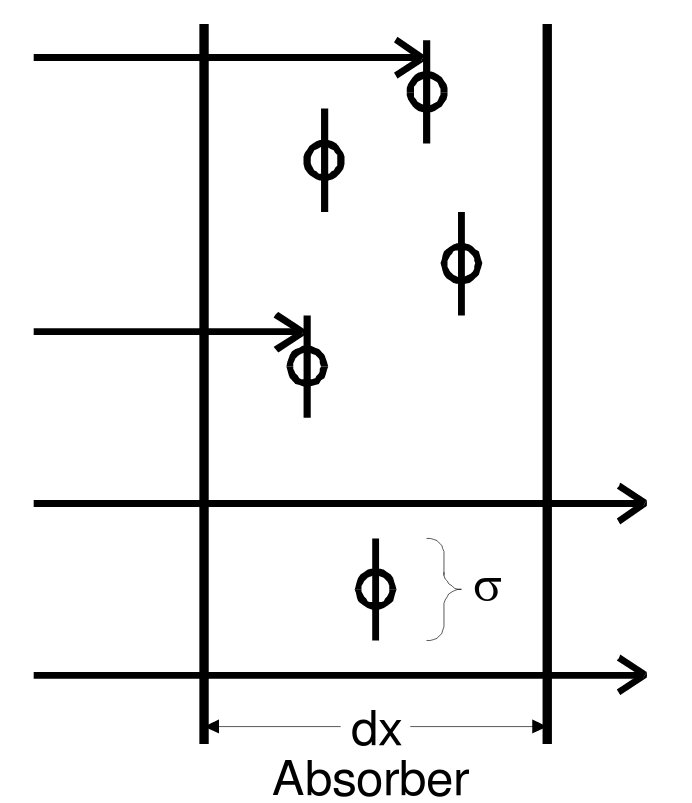
\includegraphics[width=\linewidth-250pt,height=\textheight-250pt,keepaspectratio]{content/Images/aborber.png}
    \caption{theoretische Darstellung des Wirkungsquerschnitt  \cite{V18}.}
    \label{fig:aborb}
\end{figure}

Zunächst werden die Absorptionseigenschaften von Materie bezüglich Gammastrahlung erläutert.
Wird Materie mit Gammastrahlung bestrahlt, so kommt es zu Wechselwirkungen der einzelnen Gammaquanten des Strahles mit den Atomen, Elektronen der Materie sowie den von diesen erzeugten Feldern. Desweiteren können die Quanten auch mit externen Feldern wechselwirken.%vll sind auch felder insgesamt gemeint,also auch externe
 Diese sorgen dafür, dass die Intensität des Gammastrahles entlang seines Weges durch den Festkörper abnimmt. Die drei dominierenden Effekte sind der Photoeffekt, der Comptoneffekt und die Paarbildung.
Die Wechselwirkungswahrscheinlichkeit eines jeden Effektes wird über den Wirkungsquerschnitt $\sigma$ angegeben.
% Der Beitrag der jeweiligen Wechselwirkung an der gesamten Intensitätsabnahme wird durch den zugehörigen Wirkungsquerschnitt beschrieben.
 Anschaulich lässt sich dieser als die Größe einzelner Zielscheiben deuten, welche den Einfangsradius der Atome und Elektronen beschreiben. Die Größe der Scheiben ist so gewählt, dass die Anzahl der Wechselwirkungen mit der Anzahl der verwendeten Projektilteilchen  übereinstimmt. Es wird eine infinitesimale Absorberdicke verwendet, sodass es zu keiner Überlappung der Scheiben kommt. Eine Skizze der oben genannten Vorstellung des Wirkungsquerschnitts ist in Abb. \ref{fig:aborb} dargestellt. Die Wahrscheinlichkeit, dass ein Teilchen von dem Absorber eingefangen wird, lässt sich, dem Modell gemäß, durch
 \begin{equation}
    d\text{W} = n \sigma d\text{x}
 \end{equation}
 ausdrücken. Bei $N_0$, auf den infinitisimal dicken Absorber auftreffenden, Quanten folgt für die Zahl der absorbierten Teilchen:

\begin{equation}
    d\text{N} = N_0  d\text{W} =n N_0 \sigma d\text{x}.
\end{equation}
Daraus ergeben sich für einen Absorber der Dicke $D$ mit
\begin{equation}
N(D) = N_0 \exp(-n \sigma D) \text{  bzw.  }  N_2(D) = N_0 (1 - \exp(-n \sigma D)) \label{eq:Nd}
\end{equation}
die Anzahl der wechselgewirkten Quanten $N(D)$ und die Anzahl der noch verbliebenen Quanten $N_2(D)$. Die Konstante $ \mu = n \sigma$ wird auch als Extinktionskoeffizient bezeichnet und ihr Kehrwert liefert die mittlere Reichweite der Quanten im Absorber, siehe Abb. \ref{fig:aborb}.
%wirkungsquerschnitt erläutern

\subsubsection{Photoeffekt}
Der Photoeffekt beschreibt die vollständige Absorption der Energie eines Gammaquants durch ein Hüllenelektron des Absorbers, welches daraufhin genug Energie besitzt um den Wirkungsbereich seines Kernes zu verlassen. Dafür muss die Energie des Gammaquants $E_\gamma$ größer sein als die Bindungsenergie $E_\text{B}$ des Elektrons. Aufgrund von Impulserhaltung liegen die beteiligten Elektronen meistens in der K-Schale. Die überschüssige Energie des Gammaquants wird in kinetische Energie des nun freien Elektrons umgewandelt. Der Photoeffekt lässt sich durch 
\begin{equation}
    \gamma + \text{Atom} \to \text{Atom}^+ + e^-
\end{equation}
beschreiben. Das in der Schale entstandene Loch wird anschließend durch ein Elektron einer höheren Schale gefüllt. Dieser Vorgang wiederholt sich entlang der höheren Schalen.
%auch noch nich so geil(satz links)
Die dabei frei werdenden Energien werden in Form von Röntgenquanten abgegeben. Sie verlassen den Detektor im Normalfall nicht, weswegen auch die gesamte Energie des Gammaquants im Absorber verbleibt. Dies ist im Sinne der Gammaspektroskopie wünschenwert, da sich die möglichen unterschiedlichen Zerfälle aus dem Spektrum des Photoeffekts ablesen lassen.%passt das so ,lukas fragen ob eindeutig genug
%satz sieht geklaut aus  
Der Wirkungsquerschnitt des Photoeffektes lässt sich näherungsweise durch
\begin{equation}
    \sigma_\text{ph} \propto z^\alpha E^\delta \label{eq:sigp}
\end{equation}
beschreiben. Für die Energiebereiche natürliche Strahler lassen sich $\alpha$ und $\delta$ auf $4 < \alpha <5 $ und $\delta \approx -3.5$ eingrenzen. 

\subsubsection{Comptoneffekt}

\begin{figure}
	\centering
	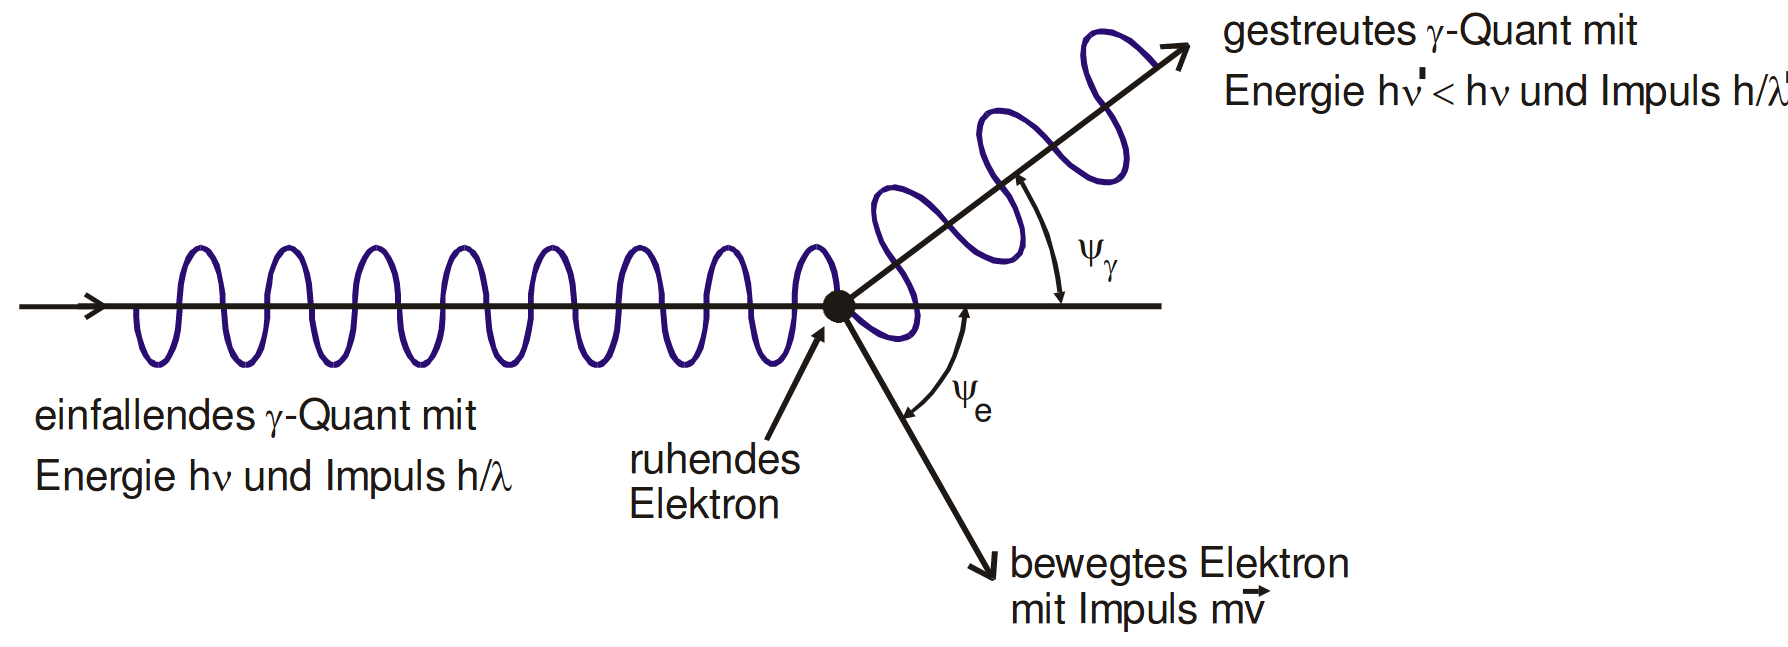
\includegraphics[width=\linewidth-100pt,height=\textheight-100pt,keepaspectratio]{content/Images/compton.png}
    \caption{Die schematische Darstellung der Comptonstreuung  \cite{V18}.}
    \label{fig:compton}
\end{figure}

\begin{figure}
	\centering
	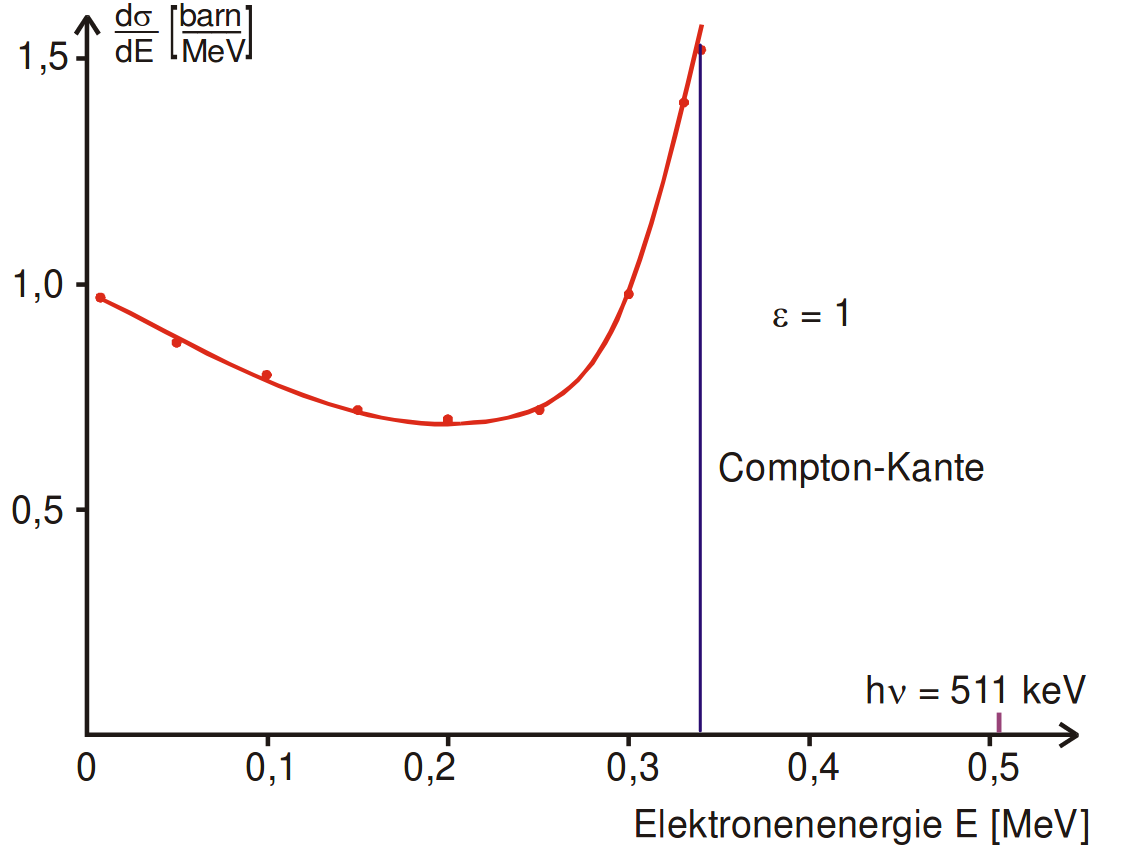
\includegraphics[width=\linewidth-100pt,height=\textheight-100pt,keepaspectratio]{content/Images/comptonk.png}
    \caption{Die Spektrumsdarstellung der Comptonkante \cite{V18}.}
    \label{fig:comptonk}
\end{figure}


Der Comptoneffekt beschreibt die unelastische Streuung eines Gammaquants an einem freien Elektron gemäß Abb. \ref{fig:compton}, wobei das Gammaquant einen Teil seiner Energie an das Elektron abgibt und seine Bewegungsrichtung ändert. Das Elektron wird näherungsweise als ruhende, punktförmige Masse angenommen. Daher lässt sich der Vorgang durch
\begin{equation}
    \gamma + e^- \to \gamma^{,} + e^{-,}
\end{equation}
beschreiben. Für die Energien gilt $E_{\gamma'} < E_\gamma$.
%Bild der comptonstreuung einfügen
Mit der Abkürzung
\begin{equation}
    \epsilon = \frac{E_\gamma}{m_e c^2} \label{eq:eps}
\end{equation}
folgen für die kinetischen Energien des Gammaquants nach dem Stoß, beziehungsweise des gestoßenen Elektrons:
\begin{equation}
    E_{\gamma'} =  E_\gamma \frac{1}{1+ \epsilon (1-\cos(\theta_\gamma))} \text{ bzw. } E_{e'} =  E_\gamma \frac{\epsilon (1-\cos(\theta_\gamma))}{1+ \epsilon (1-\cos(\theta_\gamma))} . \label{eq:ecomp}
\end{equation}
Daraus ergibt sich unter einem Streuwinkel $\theta_\gamma$ von $\SI{180}{\degree}$ ein maximaler Energieübertrag auf das Elektron von
\begin{equation}
    E_{\text{e}',\text{max}} = \frac{2 \epsilon}{1 + 2 \epsilon} E_\gamma , \label{eq:emaxcomp}
\end{equation}
welcher geringer als die Energie des Gammaquants ist. %klingt ziemlich ähnlich zur anleitung 
Aufgrund der Winkelabhängigkeit der auftretenden Energieüberträge ist der Comptoneffekt für die Gammaspektroskopie ein unerwünschter Effekt, da das Materialspezifische Spektrum der Gammastrahlung der Zerfälle durch dessen kontinuierliches Spektrum überlagert wird.%richtiges wort dafür. ist der satz eindeutig genug weil(ist diese dieses klar)
 Es zeigt sich, dass die Strahlung der Comptonstreuung keine isotrope Winkelverteilung besitzt. Für niederenergetische Gammaquanten zeigen sich Ähnlichkeiten zu einer Dipolstrahlung, bei hohen Energien oberhalb der Ruheenergie von Elektronen findet die Streuung vornehmlich in Vorwärtsrichtung statt. Für den niederenergetischen Fall mit $E_\gamma < \SI{10}{\kilo\electronvolt}$ kann der Wirkungsquerschnitt näherungsweise durch den Thomsonschen Wirkungsquerschnitt dargestellt werden und erhält
\begin{equation}
    \sigma_\text{Co} = 2 \pi r_e^2
\end{equation}
mit dem klassischen Elektronenradius $r_e$. Da der maximale Energieübertrag des Comptoneffektes geringer ausfällt, als der Peak des zugehörigen Photoeffektes, kommt es hinter dem maximalen Energieübertrag, der Comptonkante zu einer Lücke im Spektrum. Da ein Strahler in der Regel mehrere Zerfallskanäle mit unterschiedlichen Peaks besitzt, sind die Lücken im Experiment oft ohne geeignete Auswertung nicht zu erkennen.%wertend ?

Der differentielle Wirkungsquerschnitt $\frac{d \sigma}{d\text{E}}$ des Comptoneffekts besitzt die Form gemäß Abb.\ref{fig:comptonk} und lässt sich mit
\begin{equation}
    \frac{d \sigma}{d\text{E}} =  \frac{\pi r_\text{e}^2}{m_0 c^2 \epsilon^2}\left(2+\frac{E_\text{e'}}{E_\gamma - E_\text{e'}}^2 \left[ \frac{1}{\epsilon^2} +\frac{E_\gamma - E_\text{e'}}{E_\gamma} - \frac{2(E_\gamma - E_\text{e'})}{\epsilon E_\gamma} \right]\right) \label{eq:sigmacompdiff}
\end{equation}
beschreiben.

%vll bild von comptonkante +erklärung
\subsubsection{Paarbildung}
Im Falle hochenergetischer Gammaquanten mit $E_\gamma > 2 m_e c^2$ können sich diese in ein Elektron und ein Positron umwandeln. Es gilt jedoch Impulserhaltung, weshalb ein geeignetes Teilchen als Stoßpartner vorhanden sein muss, welcher den Impuls des Gammaquants aufnimmt. Dies ist meistens ein Atom, es sind aber auch Elektronen möglich. Bei letzteren ist die Rückstoßenergie, welche mit $m^{-1}$ läuft, deutlich größer, weshalb für die Paarbildung mit einem Elektron $E_\gamma > 4 m_e c^2$ erfüllt sein muss. Die überschüssige Energie des Gammaquants verteilt sich anschließend in Form von kinetischer Energie gleichmäßig auf Elektron und Positron. Auch für die Paarbildung lässt sich nur schwer ein allgemeiner Wirkungsquerschnitt abhängig von Kernladungszahl $Z$ und $E_\gamma$ angeben, da dieser aufgrund der auftretenden Coulombkräfte abhängig vom Ort in der Elektronenhülle ist, an welchem die Paarbildung stattgefunden hat. Es können jedoch Spezialfälle für verschwindende und vollständige Abschirmung der Kernkräfte angegeben werden. Für diese gilt:
\begin{equation}
    \sigma_\text{kernnah} = \alpha r_e^2 Z^2 \left( \frac{28}{9}\ln(2) \epsilon - \frac{218}{27}\right) \text{mit } \SI{10}{\mega\electronvolt} < E_\gamma \SI{25}{\mega\electronvolt} \label{eq:sigmapaar1},
\end{equation}

\begin{equation}
    \sigma_\text{kernfern} = \alpha r_e^2 Z^2 \left( \frac{28}{9}\ln\left(\frac{183}{\sqrt[3]{Z}}\right) \epsilon - \frac{218}{27}\right) \text{mit } \SI{500}{\mega\electronvolt} < E_\gamma \label{eq:sigmapaar2}.
\end{equation}
%mherer paeks bei paarbildung erklären
Da ein Peak bei der kompletten Energie des Gammaquants nur entsteht, wenn sowohl Elektron als auch Positron vom Detektor aufgenommen werden bilden sich im Spektrum mehrere Peaks aus. Dies liegt daran, dass die Positronen mit den Elektronen des Absorbers wider zu zwei Gammaquanten annihilieren können, welche den Detektor anschließend wieder verlassen können. Aufgrunddessen bildet sich zwei Peaks bei den geringeren Energie $E-\SI{511}{\kilo\electronvolt}$(SEP) und $E-\SI{1022}{\kilo\electronvolt}$(DEP) aus.  

Zusammengefasst bilden die Wirkungsquerschnitte aller betrachteter Effekte im Falle vom Germanium einen Graphen proportional zu Abb.\ref{fig:effekt} aus. %Germaniumbild einfügen

\begin{figure}
	\centering
	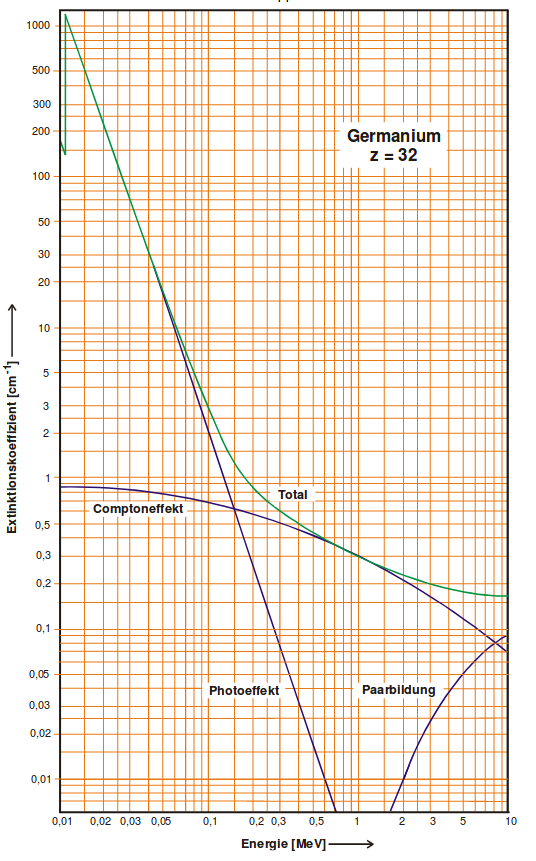
\includegraphics[width=\linewidth-100pt,height=\textheight-100pt,keepaspectratio]{content/Images/effekt.png}
    \caption{Die Energieabhängigkeit des Extinktionskoefizienten separariert nach den beteiligten Wechselwirkungen\cite{V18}.}
    \label{fig:effekt}
\end{figure}

\subsection{Die Wirkungsweise eines Reinst-Germaniumdetektors}

\begin{figure}
	\centering
    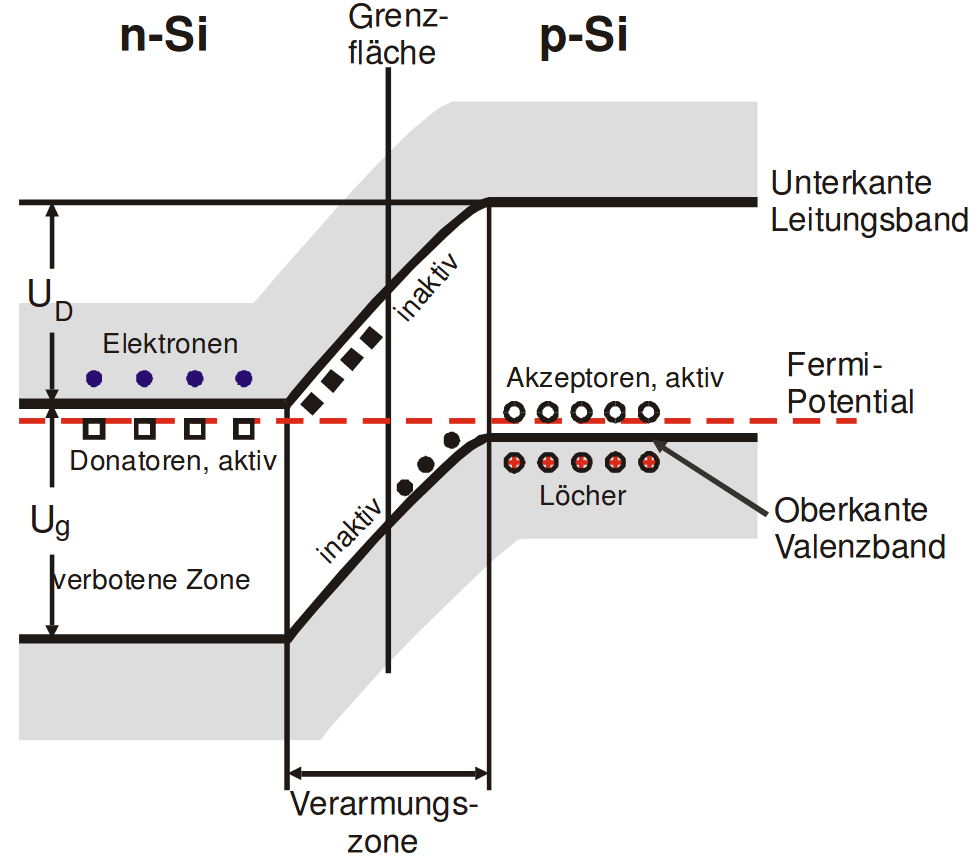
\includegraphics[width=\linewidth-200pt,height=\textheight-200pt,keepaspectratio]{content/Images/detek.png}
    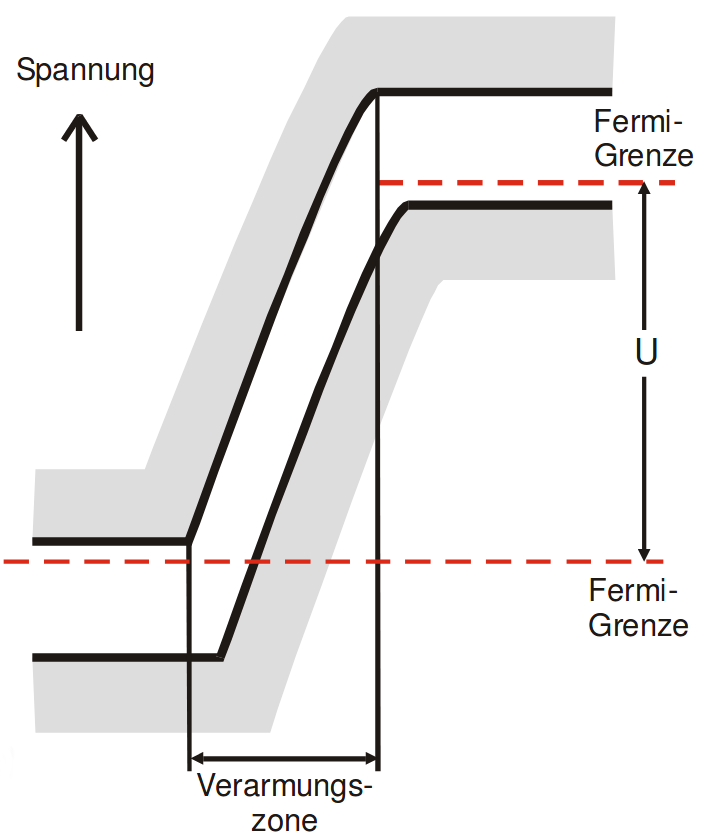
\includegraphics[width=\linewidth-200pt,height=\textheight-200pt,keepaspectratio]{content/Images/fermikante.png}
    \caption{Die schematische Darstellung der Wirkungsweise des Halbleiterdetektors\cite{V18}.}
    \label{fig:POTENTIAL}
\end{figure}
%mal sehen ob das bild passt
Die Basis des Reinst-Germaniumdetektor bildet eine Halbleiterdiode. Diese besteht aus zwei aneinandergrenzenden, unterschiedlich dotierten Materialien. Aufgrund des Ladungsträgergefälles diffundieren die beweglichen Elektronen und Löcher durch die Grenzfläche zwischen beiden Materialien hindurch und rekombinieren im Anschluss. Es verbleiben die Akzeptoren im p-dotierten und die Donatoren im n-dotierten Bereich und bilden dort eine positive bzw. negative Ladung aus. Diese erzeugen ein elektrisches Feld, welches die Bewegung der Ladungsträger wieder unterbindet. Es bildet sich eine Verarmungszone um die Grenzfläche aus. Über eine anliegende Sperrspannung lässt sich das Feld weiter verstärken, wodurch die Verarmungszone breiter wird.
%is der satz gut fragsmiley
Der ganze Vorgang wird durch ein Potentialbild nach Abb. \ref{fig:POTENTIAL} veranschaulicht. Gelangt ein Gammaquant in den Detektor und setzt ein hochenergetisches Elektron in der Verarmungszone frei, so stößt dieses auf seinem Weg durch die Verarmungszone weitere Elektronen und hebt sie aus dem Valenzband ins Leitungsband. Die entstehenden Löcher verhalten sich wie positive Ladungen. Aufgrund des in der Verarmungszone vorherrschenden elektrischen Feldes rekombinieren die Ladungsträger jedoch nicht, sondern werden anhand ihrer Ladung getrennt. Dies resultiert in einem Ladungsimpuls, welcher proportional zur Energie des gestreuten Gammaquants ist. Diese Ladungsmpulse bilden die Grundlage der Gammaspektroskopie. Daher ist es wichtig, dass möglichst viele Gammaquanten in der Verarmungszone wechselwirkungen, da nur diese Wechselwirkungen zu registrierbaren Effekten führen.% iwie is der satz immer noch nich so geil
 % da die Anzahl der gehobenen Elektron-Loch Paare von der Energie des Quants abhängt und die Höhe des Ladungsimpuls von der Anzahl der Elektron-Loch Paare.
% diese sätze sind partiell echt mies     
Da die Wahrscheinlichkeit einer Wechselwirkung des Gammaquants mit den Elektronen exponentiell von der Dicke des Materials abhängt, siehe Formel \eqref{eq:Nd}, ist es nötig eine möglichst breite Verarmungszone zu erzeugen. Diese Breite hängt von mehreren Faktoren ab.

\subsubsection{Möglichkeiten die Verarmungszone zu verbreitern}

Die Breite der Verarmungszone ist abhängig von den Dotierungen beider Bereiche. Für ihre Reichweite in den jeweilig dotierten Bereich gilt
\begin{equation}
    d_\text{n}^2 = \frac{2 \epsilon \epsilon_0}{\text{e}_0} (U_\text{D} + U) \frac{n_\text{A}}{n_\text{D}(n_\text{A}+n_\text{D})} \text{ bzw. } d_\text{p}^2 = \frac{2\epsilon \epsilon _0}{\text{e}_0} (U_\text{D} + U) \frac{n_\text{D}}{n_\text{A}(n_\text{A}+n_\text{D})} , \label{eq:d}
\end{equation}
mit der Dielektrizitätszahl $\epsilon$ und den Akzeptoren bzw. Donatorendichten $n_\text{A}$ und $n_\text{D}$.
 Um eine möglichst breite Verarmungszone zu erreichen wird daher eine sehr asymmetrische Dotierung gewählt. Daraus folgt, dass $d_\text{n}$ sehr gering ausfällt, $d_\text{p}$ hingegen sehr groß, womit die Zone durch $d_\text{p}$ allein angenähert werden kann. Da die Breite in Näherung proportional mit $\frac{1}{\sqrt{N_\text{A}}}$ verläuft, wird ein hochreiner Germaniumkristall verwendet. Eine zweite Möglichkeit die Breite zu vergrößern ist es, die anliegende Sperrspannung $U$ zu erhöhen. Die Breite wächst in diesem Fall mit $\sqrt{U}$. Allerdings kann die Spannung nicht beliebig erhöht werden. Grund hierfür sind thermische herausgelöste Elektronen, die anschließend im anliegende Feld beschleunigt werden. Die entstehenden Ströme verschlechtern die Eigenschaften des Detektors. Um die thermischen Elektronen zu reduzieren, werden der Detektor und der anliegende Vorverstärker auf ca. $\SI{77}{\kelvin}$ heruntergekühlt. Bei dieser Temperatur kann eine Spannung von $5-\SI{6}{\kilo\volt}$ angelegt werden. Mit diesen Maßnahmen wird eine Verarmungsbreite von ca. $\SI{3}{\centi\meter}$ erreicht.
 
 
\subsection{Die Eigenschaften eines Halbleiterdetektors}%nich mehr ganz so mist
Die Qualität eines Detektors wird anhand mehrerer Kenngrößen festgesetzt.
Eine wichtige Detektorkenngröße für die Spektroskopie von Gammaquanten ist das Auflösungsvermögen des Detektors. Dieses ergibt sich im wesentlichen aus der Halbwertsbreite aufgenommener Peaks einer multichromatischen Gammastrahlung. 
% passt das jetzt mit multichromatisch
Ist der Abstand der Mittelwerte zweier benachbarter Peaks mindestens so groß wie die Halbwertsbreite, so können beide Peaks unterschieden werden. Eine weitere Kenngröße ist die Höhe der Peaks. Unter der Annahme, dass ein Gammaquant, das in der Verarmungszone wechselwirkt, in dieser auch seine gesamte Energie abgibt, so folgt die Höhe des Peaks aus der Bindungsenergie und der Anzahl der erzeugten Elektron-Loch Paare. Es zeigt sich jedoch, dass die Elektron-Loch Paare nur unter Mitwirkung von Phononen entstehen. Diese werden benötigt, da Germanium ein indirekter Halbleiter ist. Die Phononen sind notwendig um bei einem Übergang den seitlichen Versatz zwischen Valenz- und Leitungsband zu überwinden. Daher verteilt sich ein Teil der Energie auf die Phononen. Für Germanium bedeutet dies, dass für ein Elektron-Loch Paar $\SI{2.9}{\electronvolt}$ benötigt werden, obwohl die Energielücke zwischen Valenz und Leitungsband nur $\SI{0.67}{\electronvolt}$ beträgt. Daher kann bei der Erzeugung nicht mehr von unkorrelierten, seltenen Ereignissen ausgegangen werden und für die Standardabweichung der zugehörigen Verteilung folgt:
\begin{equation}
\sigma = \sqrt{F \frac{E_\gamma}{E_\text{B}} }
\end{equation}
mit dem Fano-Faktor $F$. Da die aufgrund der Elektron-Loch Paar Erzeugung hervorgerufenen Fluktuationen jedoch teilweise wieder durch Fluktuationen der Phononen kompensiert werden gilt $F < 1$. Im Fall von Germanium gilt $F \approx 0.1$ \cite{V18}. Bei Betrachtung großer Zählraten kann in Näherung eine Gaußverteilung angenommen werden und die Halbwertsbreite bestimmt sich zu:
\begin{equation}
\Delta E_\text{1/2} = \sqrt{8 \ln(2) F E_\gamma E_\text{B}} \label{eq:deltE}.
\end{equation}
Die Halbwertsbreite wird jedoch durch weitere Rauscheffekte erhöht. Dazu gehören Rauschen aufgrund von Restverunreinigungen im Detektorkristall, aufgrund der angeschlossenen Verstärker und aufgrund von Imhomogenitäten im erzeugten E-Feld. Letztere folgen aus der Bauweise des Detektors. Die Effekte haben nur sehr schwache Korrelationen, sodass ihre Einflüsse in Form zusätzlicher Halbwertsbreiten quadratisch zur Ursprünglichen addiert werden können. Es gilt für die gesamte Energieauflösung $H_\text{Ges}$:
\begin{equation}
    \H_\text{Ges} = \sqrt{\Delta E_\text{1/2}^2 + H_\text{R}^2 + H_\text{I}^2 + H_\text{E}^2},
\end{equation}
mit der ungestörten Halbwertbreite $\Delta E_\text{1/2}$, der Halbwertbreite durch Leckströme $H_\text{R}$, der Halbwertsbreite aufgrund von Feldinhomogenitäten $H_\text{I}$ und der Halbwertsbreite aufgrund von Verstärkerrauschen $H_\text{E}$.
Auch in diesem Fall können die Rauscheffekte durch geringe Temperaturen minimiert werden. Im Fall der Spannung müssen Kompromisse eingegangen werden, da die Rauscheffekte sowohl bei geringen als auch bei höheren Spannungen verstärkt auftreten.

Eine letzte wichtige Kenngröße ist die Effizienz eines Detektors. Sie gibt die Energieabhängigkeit für die Wahrscheinlichkeit eines erfolgreichen Nachweis eines Gammaquants an. Aufgrund des kontinuierlichen Spektrums des Comptoneffekts ist im Energiebereich unterhalb von $\SI{3}{\mega\electronvolt}$ nur der Photoeffekt relevant. Für diesen zeigen sich theoretisch jedoch insbesondere bei höheren Energien nur geringe Vollenergienachweiswahrscheinlichkeiten. Im Experiment fallen diese jedoch höher aus. 

\subsection{Das Spektrum eines Gammastrahlers}

\begin{figure}
	\centering
	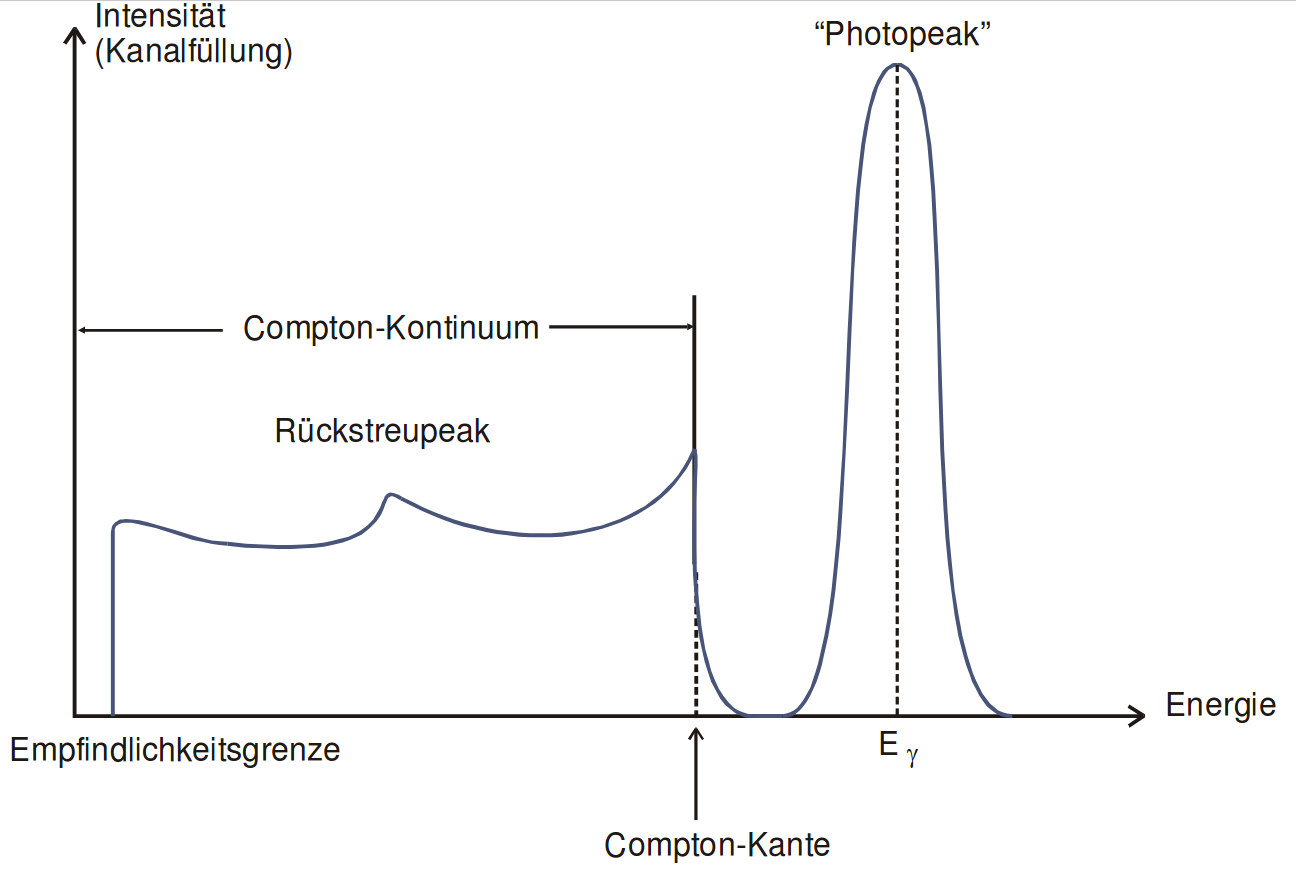
\includegraphics[width=\linewidth-100pt,height=\textheight-100pt,keepaspectratio]{content/Images/spek.png}
    \caption{Das Spektrum eines monochromatischen Gammastrahlers mit zu geringer Energie zur Paarerzeugung\cite{V18}.}
    \label{fig:spektrum}
\end{figure}

Das aufgenommene Spektrum eines Gammastrahlers besteht selbst im einfachsten Fall eines monochromatischen Strahlers nicht nur aus einem Peak, sondern besitzt eine Form gemäß Abb.\ref{fig:spektrum}. Da die Energien des Strahlers in Abb.\ref{fig:spektrum} unterhalb der Schwelle zur Paarerzeugung liegen, wird der Peak am oberen Ende der Energieskala durch den Photoeffekt hervorgerufen. Etwas unterhalb des Peak beginnt das Compton Kontinuum, welche aufgrund des Comptoneffekts auftritt. Das obere Ende des Kontinuums wird durch die Comptonkante beschrieben. Bei dieser Energie wird der Gammaquant unter einem Winkel von $\SI{180}{\degree}$ gestreut. Zusätzlich ist etwa in der Mitte des Comptonkontinuums ein weiterer Peak zu erkennen. Dieser wird Rückstreupeak genannt und entsteht, indem Elektronen die den Detektor eigentlich schon verlassen hatten unter einem Winkel von $\SI{180}{\degree}$ zurück in den Detektor gestreut werden und dort ihre nun geringere Energie mithilfe eines Photoeffekts abgeben. Der Abfall des Graphen am unteren Ende der Energieskala folgt aus der endlichen Nachweisgrenze des Detektors aufgrund der den Detektor umgebenden Aluminium-Schutzhülle. Wird ein Gammastrahler mit verschiedenen Zerfallskanälen untersucht, so kommt es zur Überlagerung der Graphen aller Kanäle. Aufgrunddessen liegen die Photopeaks der niederenergetischen Übergänge im Bereich des Compton Kontinuums der höheren Übergänge und erscheinen daher größer, weshalb der Begriff des Vollenergiepeaks passender ist. Desweiteren besitzt jeder Kanal eine unterschiedliche Zerfallswahrscheinlichkeit, was zu unterschiedlich hohen Peaks führt. Zuletzt ist auch die Effizienz des Detektors von der betrachteten Energie abhängig. All diese Aspekte verändern die Form des aufgenommenen Spektrums und sind bei einer Analyse entsprechend zu berücksichtigen. Das Zählergebnis $Z$ eines Kanals ist durch
\begin{equation}
    Z = \frac{\Omega}{4 \pi}\cdot A \cdot W \cdot Q \cdot t \label{eq:ZZZ}
\end{equation}
gegeben mit dem Raumwinkel $\Omega$, der Probenaktivität $A$, der jeweiligen Emissionenwahrscheinlichkeit eines Übergangs, der Vollenergienachweiswahrscheinlichkeit $Q$ und der Messzeit $t$. Sind $Z,\Omega,A,t$ und $W$ bekannt so lässt sich daraus $Q$ ermitteln. Für $\Omega$ gilt näherungsweise
\begin{equation}
    \frac{\Omega}{4 \pi} = 0.5 \left( 1- \frac{a}{\sqrt{a^2 + r^2}}\right) ,\label{eq:omega}
\end{equation}
mit dem Radius des Detektors $r$ und dem Abstand der Probe zum Detektor $a$. 
Bei der Aktivität eines radioaktiven Nuklides ist zudem darauf zu achten, dass sich diese über die Zeit verändert. Es gilt:
\begin{equation}
    A(t) = A_0 \cdot \exp\left(\frac{-\ln(2) t }{T_{0.5}}\right), \label{eq:AAA}
\end{equation}
mit der Halbwertszeit $T_{0.5}$.